\documentclass[t]{beamer}

\title{Software Toolkit for ML}
\date{\today}
\author{Patrick O'Hara}


\usepackage[utf8]{inputenc}
\usepackage[english]{babel}
\usepackage{graphicx}
\usepackage{hyperref}

% custom colours
\definecolor{mygreen}{RGB}{0, 100, 0}
\definecolor{myred}{RGB}{150, 0, 0}
\definecolor{myblue}{RGB}{0, 0, 100}
\newcommand{\fgreen}[1]{\textcolor{mygreen}{#1}}
\newcommand{\fred}[1]{\textcolor{myred}{#1}}
\newcommand{\fblue}[1]{\textcolor{myblue}{#1}}

\setbeamercovered{transparent=50}

\AtBeginSection[]{
  \begin{frame}
  \vfill
  \centering
  \begin{beamercolorbox}[sep=8pt,center,shadow=true,rounded=true]{title}
    \usebeamerfont{title}\insertsectionhead\par%
  \end{beamercolorbox}
  \vfill
  \end{frame}
}

\begin{document}

\begin{frame}
	\titlepage
\end{frame}

\begin{frame}{Overview}
    \tableofcontents
\end{frame}

\begin{frame}{Overview}
    \begin{block}<1>{Aims}
        \begin{itemize}
            \item Introduction to more advanced software engineering tools skills relevant to your research
            \item Collaborate on a project template we can all use in the future
        \end{itemize}
    \end{block}

    \begin{block}<2>{We are not...}
        \begin{itemize}
            \item doing an in depth tutorial for python, docker, slurm, etc.
            \item covering ML libraries such as tensoflow, pytorch, etc...
        \end{itemize}
    \end{block}

    \begin{block}<3>{Questions for later}
        \begin{enumerate}
            \item How do you set up a new project?
            \item How do you test a model?
            \item How do you set up your experiments?
        \end{enumerate}
    \end{block}
\end{frame}


\section{Getting started}
\begin{frame}{Don't over-engineer!}
    \begin{figure}
        
\includegraphics[width=0.75\linewidth]{figures/but-it-runs.jpg}
    \end{figure}
\end{frame}
\subsection{Git repo}
\begin{frame}{Getting started}
    \begin{block}<1>{Use version control}
        \begin{enumerate}
            \item Create issue
            \item Branch from main
            \item Create pull request
            \item Run tests, linting, CI
            \item Review
            \item Merge
        \end{enumerate}
    \end{block}
    \begin{block}<2>{Virtual environment}
        Environment for every project
    \end{block}

    \begin{block}<3>{Project structure}
        \href{https://github.com/warwick-machine-learning-group/pywmlg}{https://github.com/warwick-machine-learning-group/pywmlg}
    \end{block}
\end{frame}


\subsection{Python packages}


\begin{frame}{Getting started}
    \begin{block}<1>{Why use a python package?}
        \begin{itemize}
            \item Re-useable code - use in notebooks, scripts, tests, ...
            \item Break down large systems into managable modules
            \item Each module has a purpose: more readable code
        \end{itemize}
    \end{block}

    \begin{block}<2>{Dependencies}
        \begin{itemize}
            \item List in setup.py
            \item Use the most recent version of python/software
            \item Use numpy$>=1.21.0$ to specify minimum version
            \item If reproducibility is required, specify exact version: numpy==1.21.0
        \end{itemize}
    \end{block}
\end{frame}

\subsection{Conda \& virtual environments}

\section{Testing in python}

\subsection{Why test? How much to test?}

\begin{frame}{Why test?}
    \begin{figure}
        \centering
        
\includegraphics[width=\linewidth]{figures/testing_meme.png}
    \end{figure}
\end{frame}

\begin{frame}{Why test?}
    \begin{itemize}
        \item<1> To make sure your code works
        \item<2> Unit tests reduces code complexity
        \item<3> Makes your code reusable
        \item<4> Find bugs faster - especially useful for HPC! 
    \end{itemize}
    \begin{block}<5>{How much testing is too much testing?}
        Should I test every function and class?
        \begin{itemize}
            \item Critical functions should be tested
            \item Functions that are re-used frequently
            \item Functions with lots of edge cases
            \item Collaborating on a large project
        \end{itemize}
    \end{block}
\end{frame}

\subsection{Parametrized fixtures}

\begin{frame}{Testing in python: parametrized fixtures}
    \begin{block}<1>{Fixtures}
        Re-useable data/function across multiple tests
    \end{block}

    \begin{block}<2>{Parametrized fixtures}
        One testing function, lots of inputs
    \end{block}
\end{frame}

\begin{frame}{How do you test a model?}

\end{frame}

\subsection{Linting \& type hinting}

\begin{frame}{Linting}
    \begin{columns}
        \begin{column}{0.5\textwidth}
            \begin{figure}
                \centering
                
\includegraphics[width=\linewidth]{figures/linting.jpg}
            \end{figure}
        \end{column}
        \begin{column}{0.5\textwidth}
            \begin{block}<1>{Why lint?}
                Resolve basic coding errors:
                \begin{itemize}
                    \item Bad names
                    \item Unreachable code
                    \item Missing dependencies
                \end{itemize}
                ... and improves your style
            \end{block}
            \begin{block}<2>{pylint}
                Can be fussy: you can choose to only turn on errors and warnings.
            \end{block}

            \begin{block}<3>{Type hinting (mypy)}
                \begin{itemize}
                    \item Helps document your code
                    \item Validation of types
                \end{itemize}
            \end{block}
        \end{column}
    \end{columns}
\end{frame}

\section{Reproducibility}

\begin{frame}{Reproducibility - Claerbout and Karrenbach (1992)}
    \centering
    \vspace*{\fill}
    \begin{quotation}
        Authors provide all the necessary data and the computer codes to run the analysis again, re-creating the results.
    \end{quotation}
    \vspace*{\fill}
\end{frame}

\begin{frame}{Reproducibility: the Turing way}
    \centering
    \href{https://github.com/alan-turing-institute/the-turing-way}{https://github.com/alan-turing-institute/the-turing-way}
    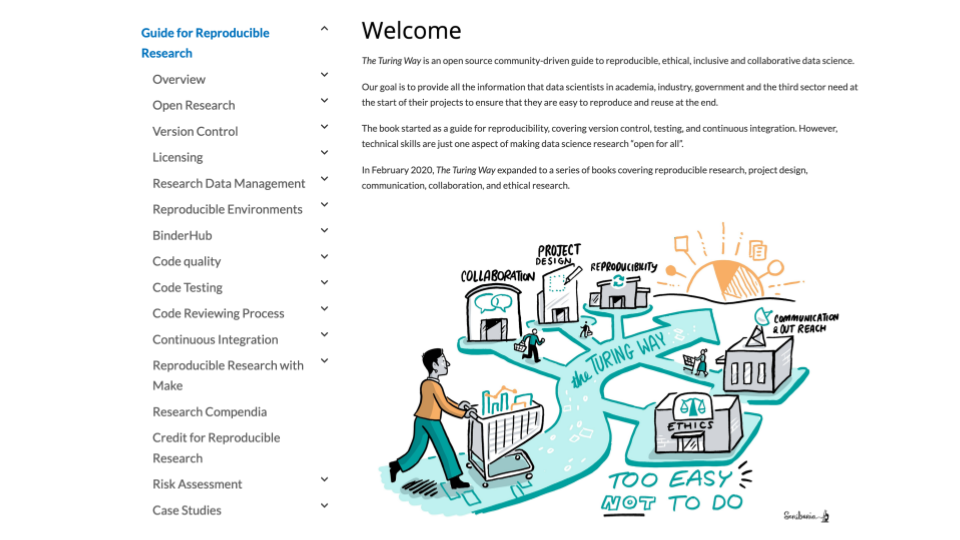
\includegraphics[width=\linewidth]{figures/TuringWay.png}
\end{frame}

\subsection{Docker}

\begin{frame}{Reproducibility - containerisation}
    \begin{block}<1>{What is a container?}
        A container is a standard unit of software that packages up code and all its dependencies so the application runs quickly and reliably from one computing environment to another. 
    \end{block}

    \begin{block}<2-8>{Why use Docker?}
        \begin{itemize}
            \item<3> Reproduce results: same dependencies, same operating system, same code
            \item<4> HPC often supports singularity: no more HPC dependency nightmares!
            \item<5> Easy for others to run your code
            \item<6> GPU support for ML libraries such as tensoflow, pytorch, etc...
            \item<7> Pull images from Docker Hub
            \item<8> Can take up a lot of storage/CPU :(
        \end{itemize}
    \end{block}
\end{frame}

\section{Continuous integration (CI)}

\begin{frame}{Continuous integration}
    Build, test, merge, deploy
    \begin{block}{Why use CI?}
        \begin{itemize}
            \item<1> Automated testing
            \item<2> Stop broken code being merged into master
            \item<3> Automated docker builds
        \end{itemize}
    \end{block}
\end{frame}

\section{Slurm}

\begin{frame}{Slurm}
    \begin{block}<1>{What is Slurm?}
        Cluster management and job scheduling system.
    \end{block}

    \begin{block}<2>{Key commands}
        \begin{itemize}
            \item sbatch: submit batch jobs
            \item squeue: see jobs in queue
            \item sinfo: see status of cluster
            \item scancel: cancel a job
        \end{itemize}
    \end{block}

    \begin{block}<3>{Slurm batch file}
        See example
    \end{block}
\end{frame}

\end{document}